\documentclass[9pt]{beamer}
\usepackage[utf8]{inputenc}
\usefonttheme{serif} 
\usefonttheme{structuresmallcapsserif} 
\usepackage{hyperref}
\hypersetup{
    colorlinks=true,
    linkcolor=blue,
    filecolor=magenta,      
    urlcolor=cyan,
}

\usetheme{Luebeck}
%\usepackage{media9}
%\usepackage{animate}
\usepackage{multimedia}
\usepackage{textpos} 

\addtobeamertemplate{frametitle}{}{%
    \begin{textblock*}{100mm}(11.75cm,-0.86cm)
        
\includegraphics[height=0.86cm,width=0.86cm]{HIPlogo.png}
    \end{textblock*}
    }
\addtobeamertemplate{frametitle}{}{%
    \begin{textblock*}{100mm}(10.89cm,-0.86cm)
        
\includegraphics[height=0.86cm,width=0.86cm]{HYlogo.jpg}
    \end{textblock*}}
\addtobeamertemplate{frametitle}{}{%
    \begin{textblock*}{100mm}(10.03cm,-0.86cm)
        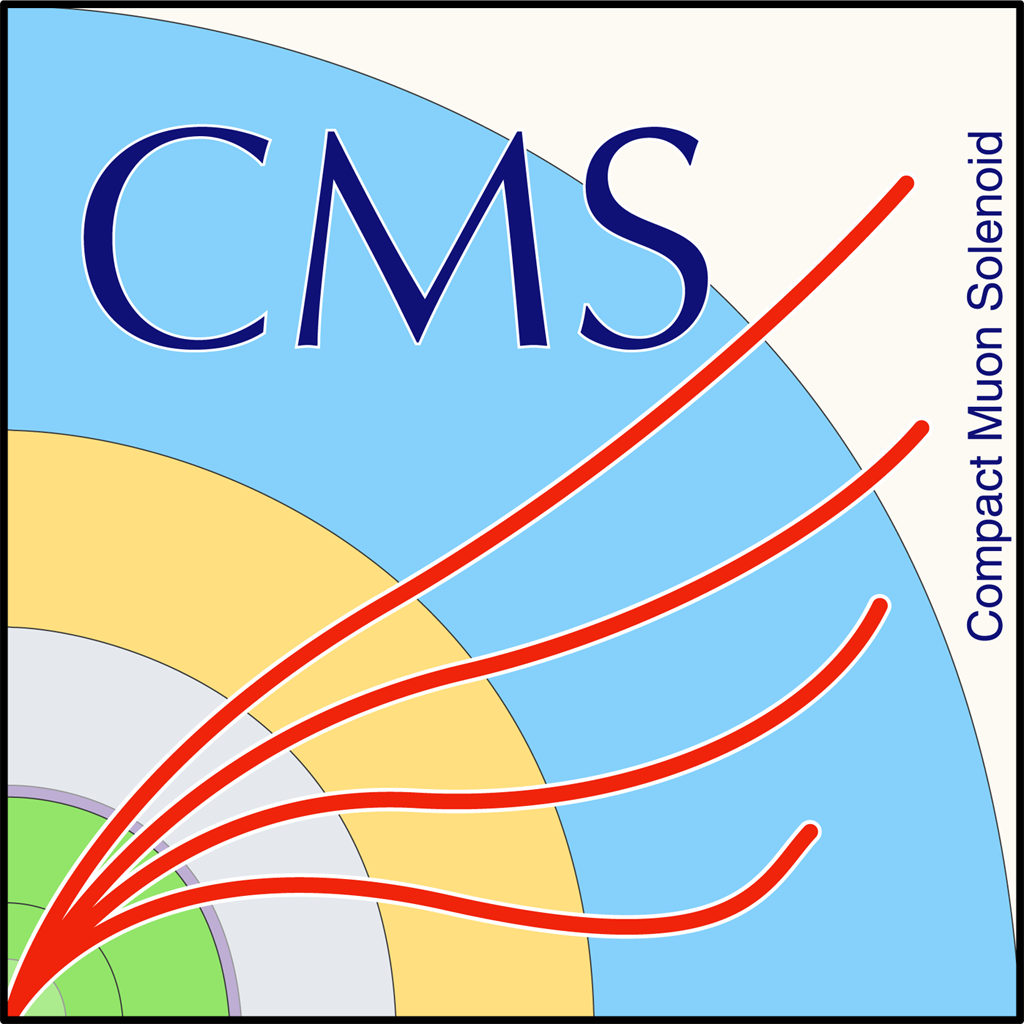
\includegraphics[height=0.86cm,width=0.86cm]{CMSlogo.png}
    \end{textblock*}}

\definecolor{ao}{rgb}{0.0, 0.5, 0.0}
\definecolor{darkgreen}{rgb}{0.0, 0.2, 0.13}
\definecolor{ferngreen}{rgb}{0.31, 0.47, 0.26}
    
\usecolortheme[named=ferngreen]{structure}
\beamertemplatenavigationsymbolsempty
\setbeamertemplate{bibliography item}[text]
\title[Legacy data (BCD16) hot zones]{Legacy data (BCD16) hot zones}
%\subtitle{JERC meeting 26th Feb 2018}
\author{Hannu Siikonen}
\institute{Helsinki Institute of Physics \\ \vspace{0.25cm} Instructor Adj.~Prof.~Mikko~Voutilainen}

\date{\today}

\setbeamersize{text margin left=5pt,text margin right=5pt}
\setlength{\labelsep}{12pt}

\begin{document}

\begin{frame}[t]
\titlepage
\end{frame}

\begin{frame}[t]{Motivation}
\begin{itemize}
 \item For the 23Sep16 ReReco we produced histograms for exlcuding ECAL hot zones
 \item More recently, there was a discussion on cleaning certain areas in HCAL \footnote{\url{https://groups.cern.ch/group/CMS-JME-L2L3Residual-Analysts/Lists/Archive/Flat.aspx?RootFolder=\%2fgroup\%2fCMS-JME-L2L3Residual-Analysts\%2fLists\%2fArchive\%2fFollow\%20up\%20on\%20HCAL\%20hot\%20towers\%20cleaning&FolderCTID=0x012002000BA29B1615BA554D933D94B87E1E3AC3}}
 \item In these slides I will present an update of the ECAL hot tower analysis - assuming now that most of the visible problems originate in the HCAL
 \item Underlying data: $\eta - \phi$ histograms of jet counts for the triggering jet of each HLT\_PFJet\* trigger separately
 \item I will be using the eras BCD for demonstration purposes (others as a reference)
 \item Definitions:
 \begin{itemize}
 \item Relative fluctuation plots show the fluctuation w.r.t. to the "pedestal", averaged over phi in each eta sector
 \item The excess/deficit plots show the deviation from the pedestal divided by the "good" rms value
 \item From the pedestal averaging and the good rms value we exclude values over 2 (initial) rms values away from the (initial) pedestal
 \item The Magenta patches: the current HCAL exclusion.
 \item The Black patches: Robert's suggestions for ECAL exclusion zones (23Sep16 ReReco)
 \item The Red patches: Mikko's suggestions for ECAL exlusion zones  (23Sep16 ReReco)
 \end{itemize}
\end{itemize}
\end{frame}

\begin{frame}[t]{HLT\_PFJet40 Njets (Data, MC)}
\begin{columns}[T]
  \begin{column}{.5\textwidth}
  \includegraphics[width=\linewidth]{../pdf/dataquality_njet_jt40.pdf}
  \end{column}
  \begin{column}{.5\textwidth}
  \includegraphics[width=\linewidth]{../pdf/mcquality_njet_jt40.pdf}
  \end{column}
\end{columns}
\end{frame}

\begin{frame}[t]{HLT\_PFJet40 Data}
\begin{columns}[T]
  \begin{column}{.5\textwidth}
  \includegraphics[width=\linewidth]{../pdf/dataquality_relfluctuation_jt40.pdf}
  \end{column}
  \begin{column}{.5\textwidth}
  \includegraphics[width=\linewidth]{../pdf/dataquality_significance_jt40.pdf}
  \end{column}
\end{columns}
\end{frame}

\begin{frame}[t]{HLT\_PFJet40 MC}
\begin{columns}[T]
  \begin{column}{.5\textwidth}
  \includegraphics[width=\linewidth]{../pdf/mcquality_relfluctuation_jt40.pdf}
  \end{column}
  \begin{column}{.5\textwidth}
  \includegraphics[width=\linewidth]{../pdf/mcquality_significance_jt40.pdf}
  \end{column}
\end{columns}
\end{frame}

\begin{frame}[t]{HLT\_PFJet60 Njets (Data, MC)}
\begin{columns}[T]
  \begin{column}{.5\textwidth}
  \includegraphics[width=\linewidth]{../pdf/dataquality_njet_jt60.pdf}
  \end{column}
  \begin{column}{.5\textwidth}
  \includegraphics[width=\linewidth]{../pdf/mcquality_njet_jt60.pdf}
  \end{column}
\end{columns}
\end{frame}

\begin{frame}[t]{HLT\_PFJet60 Data}
\begin{columns}[T]
  \begin{column}{.5\textwidth}
  \includegraphics[width=\linewidth]{../pdf/dataquality_relfluctuation_jt60.pdf}
  \end{column}
  \begin{column}{.5\textwidth}
  \includegraphics[width=\linewidth]{../pdf/dataquality_significance_jt60.pdf}
  \end{column}
\end{columns}
\end{frame}

\begin{frame}[t]{HLT\_PFJet60 MC}
\begin{columns}[T]
  \begin{column}{.5\textwidth}
  \includegraphics[width=\linewidth]{../pdf/mcquality_relfluctuation_jt60.pdf}
  \end{column}
  \begin{column}{.5\textwidth}
  \includegraphics[width=\linewidth]{../pdf/mcquality_significance_jt60.pdf}
  \end{column}
\end{columns}
\end{frame}

\begin{frame}[t]{HLT\_PFJet80 Njets (Data, MC)}
\begin{columns}[T]
  \begin{column}{.5\textwidth}
  \includegraphics[width=\linewidth]{../pdf/dataquality_njet_jt80.pdf}
  \end{column}
  \begin{column}{.5\textwidth}
  \includegraphics[width=\linewidth]{../pdf/mcquality_njet_jt80.pdf}
  \end{column}
\end{columns}
\end{frame}

\begin{frame}[t]{HLT\_PFJet80 Data}
\begin{columns}[T]
  \begin{column}{.5\textwidth}
  \includegraphics[width=\linewidth]{../pdf/dataquality_relfluctuation_jt80.pdf}
  \end{column}
  \begin{column}{.5\textwidth}
  \includegraphics[width=\linewidth]{../pdf/dataquality_significance_jt80.pdf}
  \end{column}
\end{columns}
\end{frame}

\begin{frame}[t]{HLT\_PFJet80 MC}
\begin{columns}[T]
  \begin{column}{.5\textwidth}
  \includegraphics[width=\linewidth]{../pdf/mcquality_relfluctuation_jt80.pdf}
  \end{column}
  \begin{column}{.5\textwidth}
  \includegraphics[width=\linewidth]{../pdf/mcquality_significance_jt80.pdf}
  \end{column}
\end{columns}
\end{frame}

\begin{frame}[t]{HLT\_PFJet140 Njets (Data, MC)}
\begin{columns}[T]
  \begin{column}{.5\textwidth}
  \includegraphics[width=\linewidth]{../pdf/dataquality_njet_jt140.pdf}
  \end{column}
  \begin{column}{.5\textwidth}
  \includegraphics[width=\linewidth]{../pdf/mcquality_njet_jt140.pdf}
  \end{column}
\end{columns}
\end{frame}

\begin{frame}[t]{HLT\_PFJet140 Data}
\begin{columns}[T]
  \begin{column}{.5\textwidth}
  \includegraphics[width=\linewidth]{../pdf/dataquality_relfluctuation_jt140.pdf}
  \end{column}
  \begin{column}{.5\textwidth}
  \includegraphics[width=\linewidth]{../pdf/dataquality_significance_jt140.pdf}
  \end{column}
\end{columns}
\end{frame}

\begin{frame}[t]{HLT\_PFJet140 MC}
\begin{columns}[T]
  \begin{column}{.5\textwidth}
  \includegraphics[width=\linewidth]{../pdf/mcquality_relfluctuation_jt140.pdf}
  \end{column}
  \begin{column}{.5\textwidth}
  \includegraphics[width=\linewidth]{../pdf/mcquality_significance_jt140.pdf}
  \end{column}
\end{columns}
\end{frame}

\begin{frame}[t]{HLT\_PFJet200 Njets (Data, MC)}
\begin{columns}[T]
  \begin{column}{.5\textwidth}
  \includegraphics[width=\linewidth]{../pdf/dataquality_njet_jt200.pdf}
  \end{column}
  \begin{column}{.5\textwidth}
  \includegraphics[width=\linewidth]{../pdf/mcquality_njet_jt200.pdf}
  \end{column}
\end{columns}
\end{frame}

\begin{frame}[t]{HLT\_PFJet200 Data}
\begin{columns}[T]
  \begin{column}{.5\textwidth}
  \includegraphics[width=\linewidth]{../pdf/dataquality_relfluctuation_jt200.pdf}
  \end{column}
  \begin{column}{.5\textwidth}
  \includegraphics[width=\linewidth]{../pdf/dataquality_significance_jt200.pdf}
  \end{column}
\end{columns}
\end{frame}

\begin{frame}[t]{HLT\_PFJet200 MC}
\begin{columns}[T]
  \begin{column}{.5\textwidth}
  \includegraphics[width=\linewidth]{../pdf/mcquality_relfluctuation_jt200.pdf}
  \end{column}
  \begin{column}{.5\textwidth}
  \includegraphics[width=\linewidth]{../pdf/mcquality_significance_jt200.pdf}
  \end{column}
\end{columns}
\end{frame}

\begin{frame}[t]{HLT\_PFJet260 Njets (Data, MC)}
\begin{columns}[T]
  \begin{column}{.5\textwidth}
  \includegraphics[width=\linewidth]{../pdf/dataquality_njet_jt260.pdf}
  \end{column}
  \begin{column}{.5\textwidth}
  \includegraphics[width=\linewidth]{../pdf/mcquality_njet_jt260.pdf}
  \end{column}
\end{columns}
\end{frame}

\begin{frame}[t]{HLT\_PFJet260 Data}
\begin{columns}[T]
  \begin{column}{.5\textwidth}
  \includegraphics[width=\linewidth]{../pdf/dataquality_relfluctuation_jt260.pdf}
  \end{column}
  \begin{column}{.5\textwidth}
  \includegraphics[width=\linewidth]{../pdf/dataquality_significance_jt260.pdf}
  \end{column}
\end{columns}
\end{frame}

\begin{frame}[t]{HLT\_PFJet260 MC}
\begin{columns}[T]
  \begin{column}{.5\textwidth}
  \includegraphics[width=\linewidth]{../pdf/mcquality_relfluctuation_jt260.pdf}
  \end{column}
  \begin{column}{.5\textwidth}
  \includegraphics[width=\linewidth]{../pdf/mcquality_significance_jt260.pdf}
  \end{column}
\end{columns}
\end{frame}

\begin{frame}[t]{HLT\_PFJet320 Njets (Data, MC)}
\begin{columns}[T]
  \begin{column}{.5\textwidth}
  \includegraphics[width=\linewidth]{../pdf/dataquality_njet_jt320.pdf}
  \end{column}
  \begin{column}{.5\textwidth}
  \includegraphics[width=\linewidth]{../pdf/mcquality_njet_jt320.pdf}
  \end{column}
\end{columns}
\end{frame}

\begin{frame}[t]{HLT\_PFJet320 Data}
\begin{columns}[T]
  \begin{column}{.5\textwidth}
  \includegraphics[width=\linewidth]{../pdf/dataquality_relfluctuation_jt320.pdf}
  \end{column}
  \begin{column}{.5\textwidth}
  \includegraphics[width=\linewidth]{../pdf/dataquality_significance_jt320.pdf}
  \end{column}
\end{columns}
\end{frame}

\begin{frame}[t]{HLT\_PFJet320 MC}
\begin{columns}[T]
  \begin{column}{.5\textwidth}
  \includegraphics[width=\linewidth]{../pdf/mcquality_relfluctuation_jt320.pdf}
  \end{column}
  \begin{column}{.5\textwidth}
  \includegraphics[width=\linewidth]{../pdf/mcquality_significance_jt320.pdf}
  \end{column}
\end{columns}
\end{frame}

\begin{frame}[t]{HLT\_PFJet400 Njets (Data, MC)}
\begin{columns}[T]
  \begin{column}{.5\textwidth}
  \includegraphics[width=\linewidth]{../pdf/dataquality_njet_jt400.pdf}
  \end{column}
  \begin{column}{.5\textwidth}
  \includegraphics[width=\linewidth]{../pdf/mcquality_njet_jt400.pdf}
  \end{column}
\end{columns}
\end{frame}

\begin{frame}[t]{HLT\_PFJet400 Data}
\begin{columns}[T]
  \begin{column}{.5\textwidth}
  \includegraphics[width=\linewidth]{../pdf/dataquality_relfluctuation_jt400.pdf}
  \end{column}
  \begin{column}{.5\textwidth}
  \includegraphics[width=\linewidth]{../pdf/dataquality_significance_jt400.pdf}
  \end{column}
\end{columns}
\end{frame}

\begin{frame}[t]{HLT\_PFJet400 MC}
\begin{columns}[T]
  \begin{column}{.5\textwidth}
  \includegraphics[width=\linewidth]{../pdf/mcquality_relfluctuation_jt400.pdf}
  \end{column}
  \begin{column}{.5\textwidth}
  \includegraphics[width=\linewidth]{../pdf/mcquality_significance_jt400.pdf}
  \end{column}
\end{columns}
\end{frame}

\begin{frame}[t]{HLT\_PFJet450 Njets (Data, MC)}
\begin{columns}[T]
  \begin{column}{.5\textwidth}
  \includegraphics[width=\linewidth]{../pdf/dataquality_njet_jt450.pdf}
  \end{column}
  \begin{column}{.5\textwidth}
  \includegraphics[width=\linewidth]{../pdf/mcquality_njet_jt450.pdf}
  \end{column}
\end{columns}
\end{frame}

\begin{frame}[t]{HLT\_PFJet450 Data}
\begin{columns}[T]
  \begin{column}{.5\textwidth}
  \includegraphics[width=\linewidth]{../pdf/dataquality_relfluctuation_jt450.pdf}
  \end{column}
  \begin{column}{.5\textwidth}
  \includegraphics[width=\linewidth]{../pdf/dataquality_significance_jt450.pdf}
  \end{column}
\end{columns}
\end{frame}

\begin{frame}[t]{HLT\_PFJet450 MC}
\begin{columns}[T]
  \begin{column}{.5\textwidth}
  \includegraphics[width=\linewidth]{../pdf/mcquality_relfluctuation_jt450.pdf}
  \end{column}
  \begin{column}{.5\textwidth}
  \includegraphics[width=\linewidth]{../pdf/mcquality_significance_jt450.pdf}
  \end{column}
\end{columns}
\end{frame}

\begin{frame}[t]{Cumulative summary (Data,MC)}
\begin{columns}[T]
  \begin{column}{.5\textwidth}
  \includegraphics[width=\linewidth]{../pdf/dataquality_cumulation.pdf}
  \end{column}
  \begin{column}{.5\textwidth}
  \includegraphics[width=\linewidth]{../pdf/mcquality_cumulation.pdf}
  \end{column}
\end{columns}
\begin{itemize}
 \item Cumulative summary plots over all triggers - attempt to present the excess/deficit plots cumulated over all triggers
 \item In the $\eta$ border zones only the triggers with a sufficient amount of data is used
\end{itemize}
\end{frame}

\begin{frame}[t]{Filtered cumulative summary Data (hot, cold)}
\begin{columns}[T]
  \begin{column}{.5\textwidth}
  \includegraphics[width=\linewidth]{../pdf/dataquality_hots.pdf}
  \end{column}
  \begin{column}{.5\textwidth}
  \includegraphics[width=\linewidth]{../pdf/dataquality_colds.pdf}
  \end{column}
\end{columns}
\begin{itemize}
 \item The same procedure as on the previous slide, but now we emphasize noise that is significant in more than only one trigger
 \item Hot and cold zones separated
\end{itemize}
\end{frame}

\begin{frame}[t]{Filtered cumulative summary MC (hot, cold)}
\begin{columns}[T]
  \begin{column}{.5\textwidth}
  \includegraphics[width=\linewidth]{../pdf/mcquality_hots.pdf}
  \end{column}
  \begin{column}{.5\textwidth}
  \includegraphics[width=\linewidth]{../pdf/mcquality_colds.pdf}
  \end{column}
\end{columns}
\begin{itemize}
 \item Cold zones quite well modeled in MC
 \item Hot zones not at all
\end{itemize}
\end{frame}

\begin{frame}[t]{Filtered cumulative summary MC (hot, cold)}
\begin{itemize}
 \item Hot zones are still present in the Legacy ReReco
 \item The HCAL exclusion zones are quite OK, but not completely in place
 \item The ECAL exclusion zones are mostly off, with only a couple of hits
 \item For complete results, see \footnote{\url{http://hsiikone.web.cern.ch/hsiikone/hotcoldjets/Legacy16/}}
 \item Filtered hot zone maps for each era are given as a reference for exclusion purposes
 \item The unfiltered h2hot results and the filtered h2hot results (for filtering usage) given
 \item For e.g. B,C,D these seem to be quite good substitutions for the filters
 \item Some Eras more noisy, and I would preferably use GH instead of Fl(ate)
 \item The area $\eta > 3.0$ seems to be a bit noisy in general, and needs consideration (exclusion or not)
\end{itemize}
\end{frame}

\end{document}
